% !TeX root = informe.tex
\documentclass[a4paper,11pt]{article}
\usepackage[paper=a4paper, left=3cm, right=3cm, bottom=2.5cm, top=2.5cm]{geometry}
\usepackage[spanish]{babel}
\usepackage[utf8]{inputenc}

\usepackage{caption}
\usepackage{caratula} %Paquete para usar la caratula del DC.(*You don't say?*)
\usepackage{listings}

% Esto es un """hack""" para que listings pueda mostrar carácteres especiales en el código embebido (source: https://en.wikibooks.org/wiki/LaTeX/Source_Code_Listings#Encoding_issue )
\lstset{literate=
  {á}{{\'a}}1 {é}{{\'e}}1 {í}{{\'i}}1 {ó}{{\'o}}1 {ú}{{\'u}}1,
}

\usepackage{multicol}
\usepackage{nameref}
\usepackage{natbib}
\usepackage[pdftex]{graphicx}
%\usepackage{subfigure} %Paquete para crear subfloats para poner varias imagenes en una linea -- paquete deprecado!
\usepackage[svgnames, table, usenames, dvipsnames]{xcolor}
\usepackage{tabularx}

\usepackage{geometry}
\usepackage{amsfonts}
\usepackage{graphicx}
\usepackage{verbatim}
\usepackage{float}
\parindent = 0 pt
\parskip = 11 pt

\definecolor{mygreen}{rgb}{0,0.6,0}
\definecolor{mygray}{gray}{0.25}
\definecolor{myblue}{rgb}{0.2,0.2,0.6}

%Estilos para el c\'odigo fuente
\lstset{
	basicstyle=\ttfamily\scriptsize,
	breaklines=true,
	captionpos=b,
	commentstyle=\color{mygreen},
	escapechar=@,
	extendedchars=true,
	identifierstyle=\color{myblue},
	language=C++,
	numbers=left,
	numberstyle=\tiny\color{mygray},
	stringstyle=\color{orange},	
	tabsize=3
}

\begin{document}

\titulo{Recuperatorio TP 1 - Scheduling}
\fecha{28/06/2015}
\materia{Sistemas Operativos}
\integrante{Gabriel Gramajo}{564/09}{gramajogm@gmail.com}
\integrante{Paula Jimenez}{655/10}{puly05@gmail.com}

\maketitle

\pagenumbering{arabic}
\parindent 2em %Define indentado de cada parrafo
\parskip 4pt %Define el espacio entre parrafos
\renewcommand{\baselinestretch}{1.5}

% \,
% \clearpage
% \hbox{}
% \thispagestyle{empty}
% \newpage

\tableofcontents

\setcounter{section}{0}

\newpage

\section{Introducci\'on}

\subsection{Desarrollo de ejercicios 1 y 2}
A lo largo del primer ejercicio se implementó la tarea TaskConsola, la cual consiste en realizar $n$ llamadas bloqueantes con duración al azar. La duración de dichas llamadas debe pertenecer al intervalo [bmin, bmax], lo cual se logra con la función rand().

Luego, en el siguiente ejercicio, se solicita realizar un lote de tareas. Dichas tareas deben ser: una de uso intensivo (CPU) y las restantes de uso interactivo (TaskConsola). En el uso de TaskConsola se experimentó a partir de la cantidad de bloqueos y el intervalo de tiempo que debian durar los mismos.
El bloque realizado, consiste en llamar en dos oportunidades a la tarea TaskConsola: en un principio con 3 llamadas bloqueantes de duraci\'on entre 4 y 7 milisegundos y luego con 9 llamadas bloqueantes de duraci\'on entre 5 y 15 milisegundos.
Dichas tareas se manejan bajo el criterio del Scheduler FCFS (First Come, First Served). El cual consiste en dar lugar a la ejecuci\'on de la tarea que llegue primero.
Se realizaron pruebas para 1 y 2 n\'ucleos dado que el scheduler acepta multicore. El comportamiento de las tareas se observa a continuación:

\begin{figure}[H]
\centering
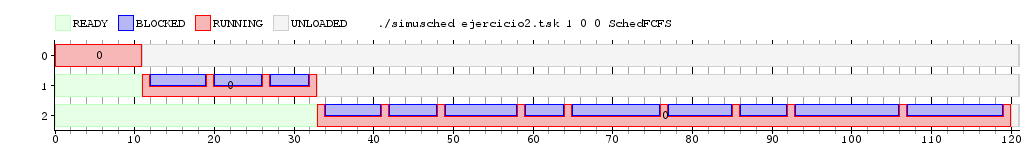
\includegraphics[scale=.6, width=1\textwidth]{graficos/ej2-1core}
\caption{Gráfico con tres tareas y un core}
\end{figure}

En el presente gráfico ingresan tres tareas las cuales: la primera no contiene bloqueos, la segunda tarea entrante contiene tres bloqueos con duración elegida al azar y la última tarea leida contiene nueve bloqueos. Ninguna de las tareas, más allá de sus bloqueos es interrumpida ya que el scheduler utilizado es FCFS. 

Luego, en el gráfico que se presenta a continuación podemos observar que teniendo dos cores el tiempo de ejecución de las tareas se reduce considerablemente. Cabe destacar que en ambos gráficos las duraciones de los bloqueos son realmente al azar. 

\begin{figure}[H]
\centering
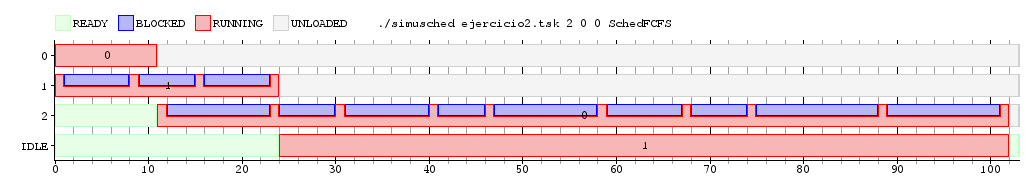
\includegraphics[scale=.6, width=1\textwidth]{graficos/ej2-2core}
\caption{Gráfico con tres tareas y dos cores}
\end{figure}


\pagebreak

\section{Ejercicio 3}
	\subsection{Introducción}
		En este ejercicio se pidió que se implementara un scheduler basado en el algoritmo Round-Robin. El mismo debía brindar soporte para el uso de multiples procesadores.
		
		Round-Robin es uno de los algoritmos usados comunmente para el scheduling de procesos, principalmente en sistemas interactivos, es decir, aquellos sistemas que requieren que se responda rápidamente los pedidos del usuario. 

	\subsubsection*{Algorítmo Round-Robin}
		Este es uno de los algoritmos más antiguos, simples, justos\footnote{Ver concepto de fairness en la Sección 1.} y más ampliamente usados. A cada proceso se le es asignado un intervalo de tiempo, denominado \textbf{quantum}, durante el cual se le permite utilizar el procesador. Si el proceso aún esta corriendo al final de su quantum, entonces se lo desaloja y se pasa a ejecutar otro proceso. Si el proceso se bloqueó o terminó de ejecutar antes de que termine su quantum, el reemplazo se realiza al momento del bloqueo o terminación. 
	
		Éste es un algoritmo fácil de implementar, lo único que necesita hacer el scheduler es mantener una lista de los procesos que están listos para ejecutar. Cuando un proceso consume todo su quantum o vuelve de un bloqueo, se lo vuelve a encolar al final de la lista.
		
		En el caso de sistemas con multiples procesadores existen al menos dos implementaciones posibles.
	
		\begin{itemize}
			\item \emph{Colas Multiples}: Cada procesador posee su propia cola de procesos a ser ejecutados. Es posible permitir o no la migración de procesos entre distintos procesadores.
			\item \emph{Cola Única}: Todos los procesadores comparte una cola de procesos a ser ejecutados. Cuando un procesador debe ejecutar un nuevo proceso, toma el primero de la cola. Esta implementación permite la migración de procesos de un procesador a otro.
		\end{itemize}
	
	\subsection{Resolución}
		\subsubsection*{Estructura Interna}
			Siguiendo el requerimiento del ejercicio implementamos un scheduler Round-Robin con una cola única de procesos para permitir la migración de los mismos entre distintos procesadores.
			La estructura interna de nuestra implementación es la siguiente:
			\lstinputlisting[name=RR1, numbers=left, frame=lines, firstline=22, lastline=25]{../src/sched_rr.h}

			\begin{enumerate}
				\item \emph{\textbf{quantums:}} vector indexado por número de procesador en el cual almacenamos el quantum inicial de cada procesador. Utilizamos un vector para poder acceder de forma directa a cada quantum.
				\item \emph{\textbf{cuota\_actual:}} almacena, para cada procesador, cuanto quantum le queda por consumir al proceso que está ejecutando. La razón por la cual utilizamos un vector es la misma que para el item anterior, acceder de manera directa al dato de un procesador dado.
				\item \emph{\textbf{cola\_procesos:}} ésta es la cola global de procesos que están esperando para ser ejecutados. Utilizamos una cola porque necesitamos mantener un orden en el cual los procesos serán ejecutados.
				\item \emph{\textbf{bloquedas:}} éste es el conjunto de procesos que se encuentran bloqueados. Utilizamos un conjunto porque no necesitabamos mantener un orden relativo entre los procesos bloqueados.
			\end{enumerate}

			\lstset{
				tabsize=1, % tabs mas chicos para el código
				aboveskip=15pt, % Espacio arriba de un bloque de código
				belowskip=15pt, % Espacio abajo de un bloque de código
			}
	
			Ésta estructura es inicializada en el contructor de la clase del scheduler.
			\lstinputlisting[name=RR1load, numbers=left, frame=lines, firstline=10, lastline=18]{../src/sched_rr.cpp}		
			
			Primero tomamos el parámetro de la cantidad de cores que tendrá el sistema y luego usamos ese dato para iterar sobre los siguientes parametros. Estos parámetros sin agregados uno a uno en el vector correspondiente.
			\\
	
			A continuación pasamos a explicar los detalles de implentación de cáda uno de los métodos que debíamos implementar.
		
		\subsubsection*{Método load}
			La carga de un proceso es bastante simple, sólamente encolamos el pid del nuevo proceso en la cola para que espere a ser ejecutado.
	
			\lstinputlisting[name=RR1load, numbers=left, frame=lines, firstline=24, lastline=27]{../src/sched_rr.cpp}	
		
		\subsubsection*{Método unblock}
			Al momento de desbloquear un proceso, borramos su pid del conjunto de tareas bloqueadas y luego lo encolamos nuevamente en la cola de procesos.
			
			\lstinputlisting[name=RR1unblock, numbers=left, frame=lines, firstline=28, lastline=31]{../src/sched_rr.cpp}
	
		\subsubsection*{Método tick}
			El siguiente método, tick, es ligeramente más complejo así que lo describiremos con algo más de detalle.	
			
			Básicamente en este método debemos responder según el motivo por el cual la función fue invocada, así que utilizamos una estructura de switch y tratamos cada motivo por separado.
			
			\lstinputlisting[name=RR1tick, numbers=left, frame=lines, firstnumber=auto, firstline=33, lastline=42]{../src/sched_rr.cpp}
			
			En el caso de que el motivo del llamado es porque se dio un tick del clock primero vemos si se está ejecutando la tarea IDLE y tenemos proceso en espera para ejecutar (linea 7). Si es así, resetamos el quantum y elegimos el próximo proceso a ejecutar (lineas 8 y 9).
		
			\lstinputlisting[name=RR1tick, numbers=left, frame=lines, firstnumber=last, firstline=43, lastline=54]{../src/sched_rr.cpp}
			
			Si la tarea que estaba ejecutando al momento del tick no era la IDLE, entonces disminuimos su cuota actual en ese procesador (linea 12).
			Si a la tarea se le agotó el quantum entonces la desalojamos y la encolamos al final de la cola de procesos (lineas 13 y 14). Esto es lo que genera la rotación de los procesos que ejecutan en ese CPU. A continuación reiniciamos el quantum para ese procesador y elegimos el próximo proceso que pasará a ejecutar (lineas 15 a 17).
			
			En el caso que la tarea no haya consumido todo su quantum, simplemente la dejamos seguir ejecutando (lineas 18 a 20).	
			
			El siguiente motivo por el cual el scheduler es llamado es el caso en que un proceso realiza una llamada bloqueante.
		
			\lstinputlisting[name=RR1tick, numbers=left, frame=lines,firstnumber=last, firstline=55, lastline=59]{../src/sched_rr.cpp}
		
			En este caso lo primero que debemos hacer es efectivamente bloquear al proceso, agregandolo al conjunto de procesos bloqueados (linea 24). Luego reiniciamos el quantum para el CPU que lo estaba corriendo y elegimos el siguiente proceso a ejecutar (lineas 25 y 26).
			\\
			
			El último caso es cuando una tarea avisa que ha terminado su ejecución. En este caso simplemente reseteamos el quantum del procesador y elegimos el siguiente proceso a ejecutar (lineas 29 y 30).
			
			\lstinputlisting[name=RR1tick, numbers=left, frame=lines,firstnumber=last, firstline=60, lastline=65]{../src/sched_rr.cpp}
			
			El método tick debe devolver el pid de la próxima tarea a ejecutar luego de la llamada al scheduler y, por lo que hemos visto antes, cada case define dicho pid antes de terminar, el cual es devuelto al final del método.

		\subsubsection*{Método next}
			Éste es el método encargado de elegir, dado un CPU, cual sería el próximo proceso a ejecutar.
	
			\lstinputlisting[name=RR1next, numbers=left, frame=lines, firstline=68, lastline=77]{../src/sched_rr.cpp}
			
			Por defecto devolvemos la tarea IDLE (linea 2). Pero si la cola de procesos no está vacía, desencolamos el primero de la cola y lo devolvemos (lineas 3 a 7).

\section{Ejercicio 4}
En el presente ejercicio, se solicita el diseño de un lote de tareas en el cual podamos justificar que el comportamiento del Scheduler implementado anteriormente es el correcto. Para esto se pens\'o en tareas de uso intensivo y as\'i tambi\'en bloqueantes en las cuales confirmaremos que se hace uso correcto del quantum dado y se respeta el valor de cambio de contexto.

\subsection{Bloque de tareas corriendo en un procesador con un n\'ucleo:}

\begin{figure}[H]
\centering
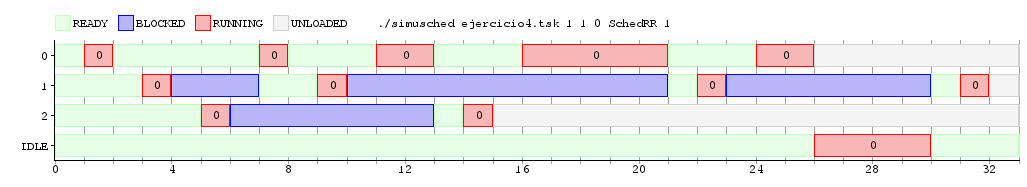
\includegraphics[scale=.6, width=1\textwidth]{graficos/ej4-1core-q}
\caption{Gráfico con tres tareas y un core}
\end{figure}

Ingresan tres tareas, teniendo un quantum de solo t = 1 (donde t es el tiempo) las tareas cumplen dicho tiempo y quedan en espera. Dado que el cambio de contexto tambien es t = 1, cada tarea demora un t en comenzar a ejecutar cuando toca su turno. Luego, al tener tareas interactivas y estar las mismas en periodo de bloqueo, las de uso intensivo tienen la posibilidad de ejecutar m\'as del quantum que le corresponde como sucede entre en los instantes 12 y 13, 16 y 21, y 24 y 26.

\subsection{Bloque de tareas corriendo en un procesador con dos n\'ucleos:}

\begin{figure}[H]
\centering
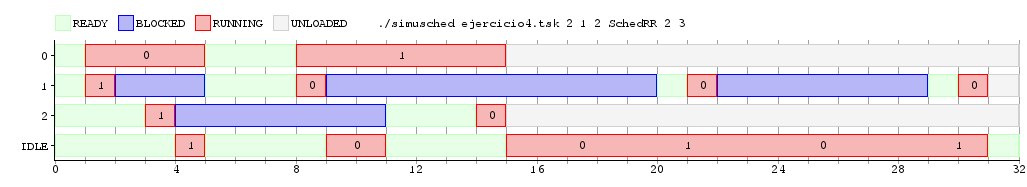
\includegraphics[scale=.6, width=1\textwidth]{graficos/ej4-2cores-q+m}
\caption{Gráfico con tres tareas y dos cores}
\end{figure}

Al tener dos n\'ucleos, se le agrega valor de migraci\'on de un n\'ucleo a otro. Las tareas se reparten en ambos y estando dos de las tareas bloqueadas, el proceso cero (que es de uso intensivo) consume su quantum y puede seguir ejecutando. Luego, el proceso uno termina su periodo de bloqueado y migra hacia el primer n\'ucleo. Es importante notar que le cuestra tres inst\'antes de tiempo ya que, dos son para migrar y el restante es de cambio de contexto. 


\section{Ejercicio 5}
Articulo: Liu, Chung Laung, and James W. Layland. Scheduling algorithms for multiprogramming
in a hard-real-time environment. Journal of the ACM (JACM) 20.1 (1973): 46-61.

\subsection{Algoritmos de prioridades fijas y din\'amicas}

En dicho art\'iculo los autores intentan resolver el problema de el uso de varias tareas en un solo procesador. Dado que hay tareas que necesitan servicio garantizado del procesador. 
En miras de este problema se estudia la utilizaci\'on de prioridades fijas con las que se lograr\'ia una utilizaci\'on del procesador de un 70 porciento para conjuntos grandes de tareas. Dicho algoritmo consiste en asignar a cada tarea como prioridad el periodo con el que llegan al procesador para jecutarse.
As\'i tambi\'en, se estudia otro algoritmo mediante el cual se puede lograr la utilizaci\'on completa del procesador. El mismo consiste en asignar dinámicamente prioridades sobre la base de sus deadlines.

%\subsection{Algoritmo de la secci\'on 7}



%\subsection{Teorema 7}



\section{Ejercicio 6}

En este ejercicio se crea un nuevo tipo de tarea, llamado TaskBatch que recibe los parámetros \emph{total\_cpu} y \emph{cant\_bloqueos}. La misma debe realizar \emph{cant\_bloqueos} llamadas bloqueantes de un ciclo de duración en momentos pseudoaleatorios y todo el tiempo de CPU que utilice la tarea, no puede superar el valor de \emph{total\_cpu}.

Para lograr esto, se le resta uno a \emph{total\_cpu} para tener en cuenta el costo del exit y luego se hace $\emph{total\_cpu} - \emph{cant\_bloqueos}$ en cada ciclo para poder elegir aleatoriamente cuanto tiempo de CPU ejecutar, sin el riesgo de quedarse sin tiempo para hacer las llamadas bloqueantes. Esto se repite mientras quede tiempo de CPU por consumir. En el caso que este se acabe y no se hayan realizado todas las llamadas bloqueantes, las mismas se ejecutan una atrás de la otra.


\pagebreak

\section{Ejercicio 7}
Para este punto, vamos a tomar las métricas turnaround y eficiencia para tratar de concluir cual es el valor óptimo de quantum para cada una.

\subsection{Turnaround}
El turnaround time se define como el intervalo que va desde el tiempo en que se carga la tarea, hasta que termina de ejecutarse. Lo que significa que para obtener este valor hay que sumar el tiempo de espera para cargarse en memoria, el tiempo de espera en la cola de ready, el tiempo de ejecución de CPU y el tiempo en estado bloqueado.

Para analizar esta métrica, armamos un lote de tareas TaskBatch con 10 ciclos de ejecución de CPU y un valor entre 1 y 8 de cantidad de bloqueos. Este lote lo corrimos con el scheduller round robin para 1, 2 y 3 cores con quantums fijos para todos los cores de 2, 5, 8 y 15.

\begin{figure}[H]
\centering
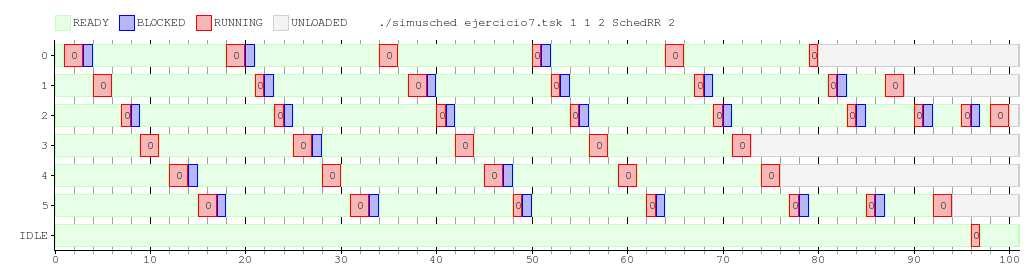
\includegraphics[scale=.6, width=1\textwidth]{graficos/ej7-1core-q1}
\caption{Gráfico con quantum 2 en un solo core}
\end{figure}

\begin{figure}[H]
\centering
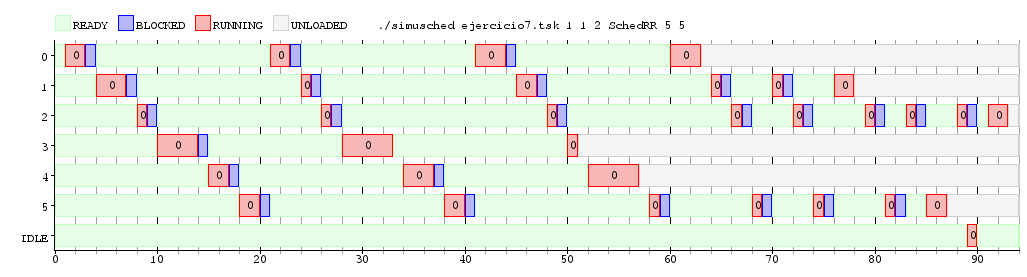
\includegraphics[scale=.6, width=1\textwidth]{graficos/ej7-1core-q2}
\caption{Gráfico con quantum 5 en un solo core}
\end{figure}

\begin{figure}[H]
\centering
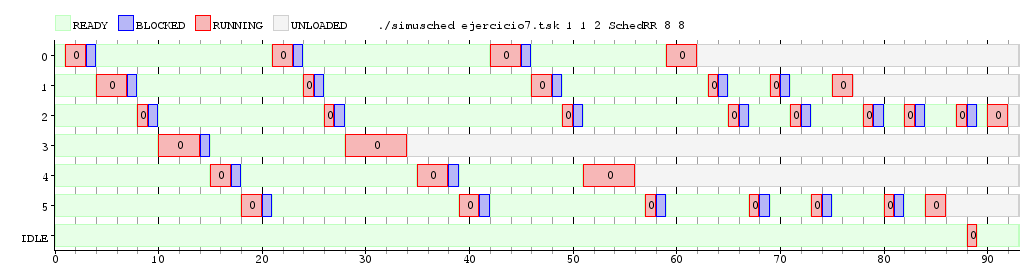
\includegraphics[scale=.6, width=1\textwidth]{graficos/ej7-1core-q3}
\caption{Gráfico con quantum 8 en un solo core}
\end{figure}

\begin{figure}[H]
\centering
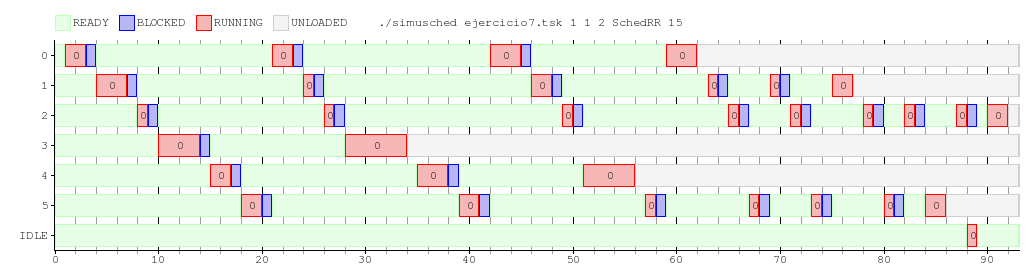
\includegraphics[scale=.6, width=1\textwidth]{graficos/ej7-1core-q4}
\caption{Gráfico con quantum 15 en un solo core}
\end{figure}

Si se analisan los gráficos se puede ver que a partir de quantum 8 no cambia el turnaround.

%\subsection{Eficiencia} 
\pagebreak

\section{Ejercicio 8}
	\subsection{Introducci\'on}
		En este ejercicio se pidió que se implementara un scheduler basado en el algoritmo Round-Robin pero, a diferencia de la implementación requerida para el \textbf{ejercicio 3}, esta implementación no debía permitir la migración de procesos entre núcleos.
		
		Éste último requerimiento básicamente nos pide que exista \emph{afinidad} de un proceso con su procesador.
		Existe una afinidad a un procesador cuando tratamos de utilizar el mismo procesador para ejecutar un proceso, aunque podamos tardar más tiempo en obtenerlo. Si esto se hace de manera estricta decimos que hay \emph{afinidad dura}. Si esta condición es más relajada decimos que hay una \emph{afinidad blanda}.
		
		Como no debemos permitir la migración entre procesos, debemos implementar un scheduler que imponga una afinidad dura.
		
		Además tenemos otra condición que es que debemos respetar un criterio al momento de elegir el procesador al que le asignaremos la siguiente tarea a ejecutar. Este critero es elegir el procesador que tenga menor carga tenga, es decir que tenga la menor cantidad de procesos activos.
		
	\subsection{Resolución}
		\subsubsection*{Estructura Interna}
			La estructura interna que usamos para implementar este scheduler es la siguiente:

			\lstinputlisting[name=RR1next, numbers=left, frame=lines, firstline=22, lastline=31]{../src/sched_rr2.h}
			
			\begin{enumerate}
				\item \emph{\textbf{cpu\_data:}} ésta estructura es un contenedor de otras que nos servirán para llevar cuenta del estado de un procesador.
				\begin{enumerate}
					\item \emph{\textbf{initial\_quantum:}} guarda el quantum inicial de un procesador.
					\item \emph{\textbf{quantum\_left:}} guarda el quantum restante. Es decir el tiempo de procesador que aún puede aprovechar un proceso.
					\item \emph{\textbf{ready\_queue:}} ésta es la cola de procesos a ejecutar.
					\item \emph{\textbf{blocked\_set:}} éste es el conjunto de procesos que se encuentran bloqueados.
				\end{enumerate}
				\item \emph{\textbf{cpus:}} este vector almacena la estructura \textit{cpu\_data} correspondiente a cada procesador.
				\item \emph{\textbf{pids\_cpu:}} este diccionario nos permite mantener un registro de la relación de un proceso con su procesador asignado.
			\end{enumerate}
			
			Ésta estructura se inicializa en con contructor de la clase del scheduler.

			\lstinputlisting[name=RR1next, numbers=left, frame=lines, firstline=9, lastline=18]{../src/sched_rr2.cpp}

			En primer lugar tomamos la cantidad de cores que recibimos por parámetro e iteramos el resto de los otros parámetros. En cada iteración creamos un \textit{cpu\_data} con los datos de quantum inicial y quantum restante para luego agregarlo a nuestro vector de cpus.\\
			
			Veamos ahora los detalles de implementación de los métodos que tuvimos que implementar.
			
		\subsubsection*{Método load, get\_unloaded\_cpu y cpu\_load}
			Al momento de cargar un nuevo proceso debemos obtener el procesador que menor carga tenga, según el criterio mencionado anteriormente. Luego encolamos el proceso el dicho procesador.
	
			\lstinputlisting[name=RR1next, numbers=left, frame=lines, firstline=22, lastline=26]{../src/sched_rr2.cpp}			
			
			Por último guardamos a qué procesador fue asignado el nuevo proceso. Esto lo necesitaremos al momento de desbloquear un proceso ya que necesitamos saber en qué procesador estaba corriendo.
			
			Para obtener el procesador con menos carga, simplemente buscamos el mínimo en nuestro vector de cpus.
	
			\lstinputlisting[name=RR1next, numbers=left, frame=lines, firstline=84, lastline=90]{../src/sched_rr2.cpp}
			
		\subsubsection*{Método tick y remove\_pid}
			Esta implementación de tick es practicamente igual a la del scheduler del \textbf{ejercicio 3} con una particularidad al momento de terminar una tarea.
	
			\lstinputlisting[name=RR1next, numbers=left, frame=lines, firstline=65, lastline=69]{../src/sched_rr2.cpp}
			
			En la linea 2 llamamos a \textit{remove\_pid}, método que borra el registro de a cual procesador estaba asociado el proceso.
	\subsection{Evaluación comparativa de Round-Robin y Round-Robin 2}
		Para comparar ambos algoritmos decidimos evaluarlos tomando en cuanta dos métricas en particular, estas son el uso de cpu y el turnaround. En segundo plano podremos ver como estos algoritmos manejan de manera el balanceo de carga del sistema de manera diferente.
		
		\subsubsection{Experimento 1}
		Para este experimento buscamos explotar lo que consideramos una deficiencia para el algoritmo que no permite la migración.
		Recordemos que para dicha implementación de Round-Robin el criterio para determinar a qué CPU se asocia un proceso es el de elegir aquél que posea cargá minima, siendo la definición de carga la siguiente:
		\begin{center}
			$carga\_cpu = RUNNING + BLOCKED + READY$
		\end{center}

		Donde RUNNING, BLOCKED y READY son los conjuntos de procesos corriendo, bloqueado y listo, respectivamente.
		Ahora bien, podría darse en caso en que en un lote de tareas varias de ellas sean intesivas en el uso de I/O y estas sean asignadas al mismo CPU. En esta situación dicho CPU pasaría la mayor parte de tiempo a la espera de que las tareas terminen de realizar su operacion de I/O y el scheduler no lo consideraría en primer lugar al de asignar una tarea intensiva en el uso de CPU.
		
		Para mostrar esta situación diseñamos un lote de pares de tareas, cada par consiste en una tarea intensiva en uso de I/O y la otra en uso de CPU. Realizamos el experimento utilizando 2 cores, tiempo de context switch de una unidad y tiempo de migración de una unidad.
		
		\begin{figure}[H]
		\centering
		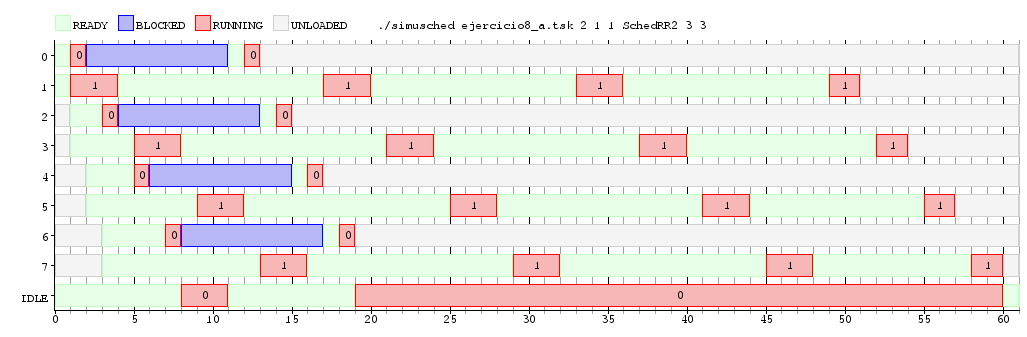
\includegraphics[scale=.4, width=1\textwidth]{graficos/ej8-a2-2c}
		\caption{SchedRR2 (sin migración)}
		\end{figure}
		
		En este caso el turnaround promedio es:\\
		
		\begin{math}
 			turnaround_{RR2} = \frac{(13-0)+(51-0)+(15-1)+(54-1)+(17-2)+(57-2)+(19-3)+(60-3)}{8} = 34,25
		\end{math}
		\\

		Por otra parte el siguiente diagrama muestra la ejecución del mismo lote para el algoritmo que si permite la migración.
		
		\begin{figure}[H]
		\centering
		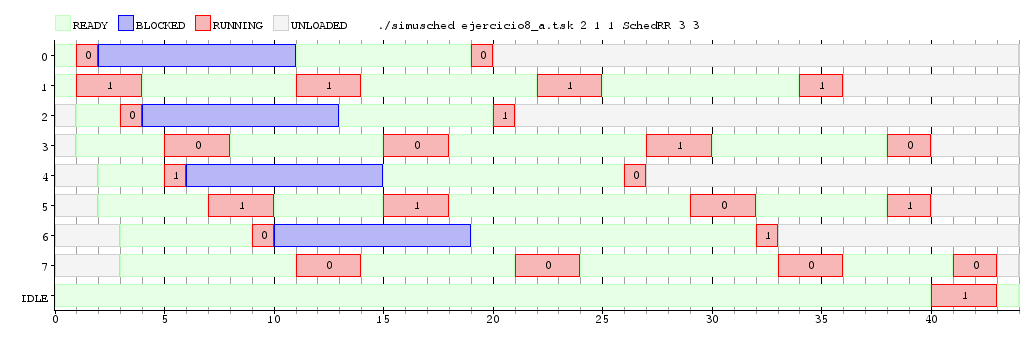
\includegraphics[scale=.4, width=1\textwidth]{graficos/ej8-a1-2c}
		\caption{SchedRR (con migración)}
		\end{figure}

		Y en este caso tenemos un turnaround promedio de:\\
		
		\begin{math}
			turnaround_{RR} = \frac{(20-0)+(36-0)+(21-1)+(40-1)+(27-2)+(40-2)+(33-3)+(43-3)}{8} = 31
		\end{math}
		\\
	
		que, tal como esperábamos, es menor que el de la implementación sin migración.
		
		Veamos el uso que hace cada algoritmo de sus  cores.
		
		\begin{figure}[H]
		\centering
		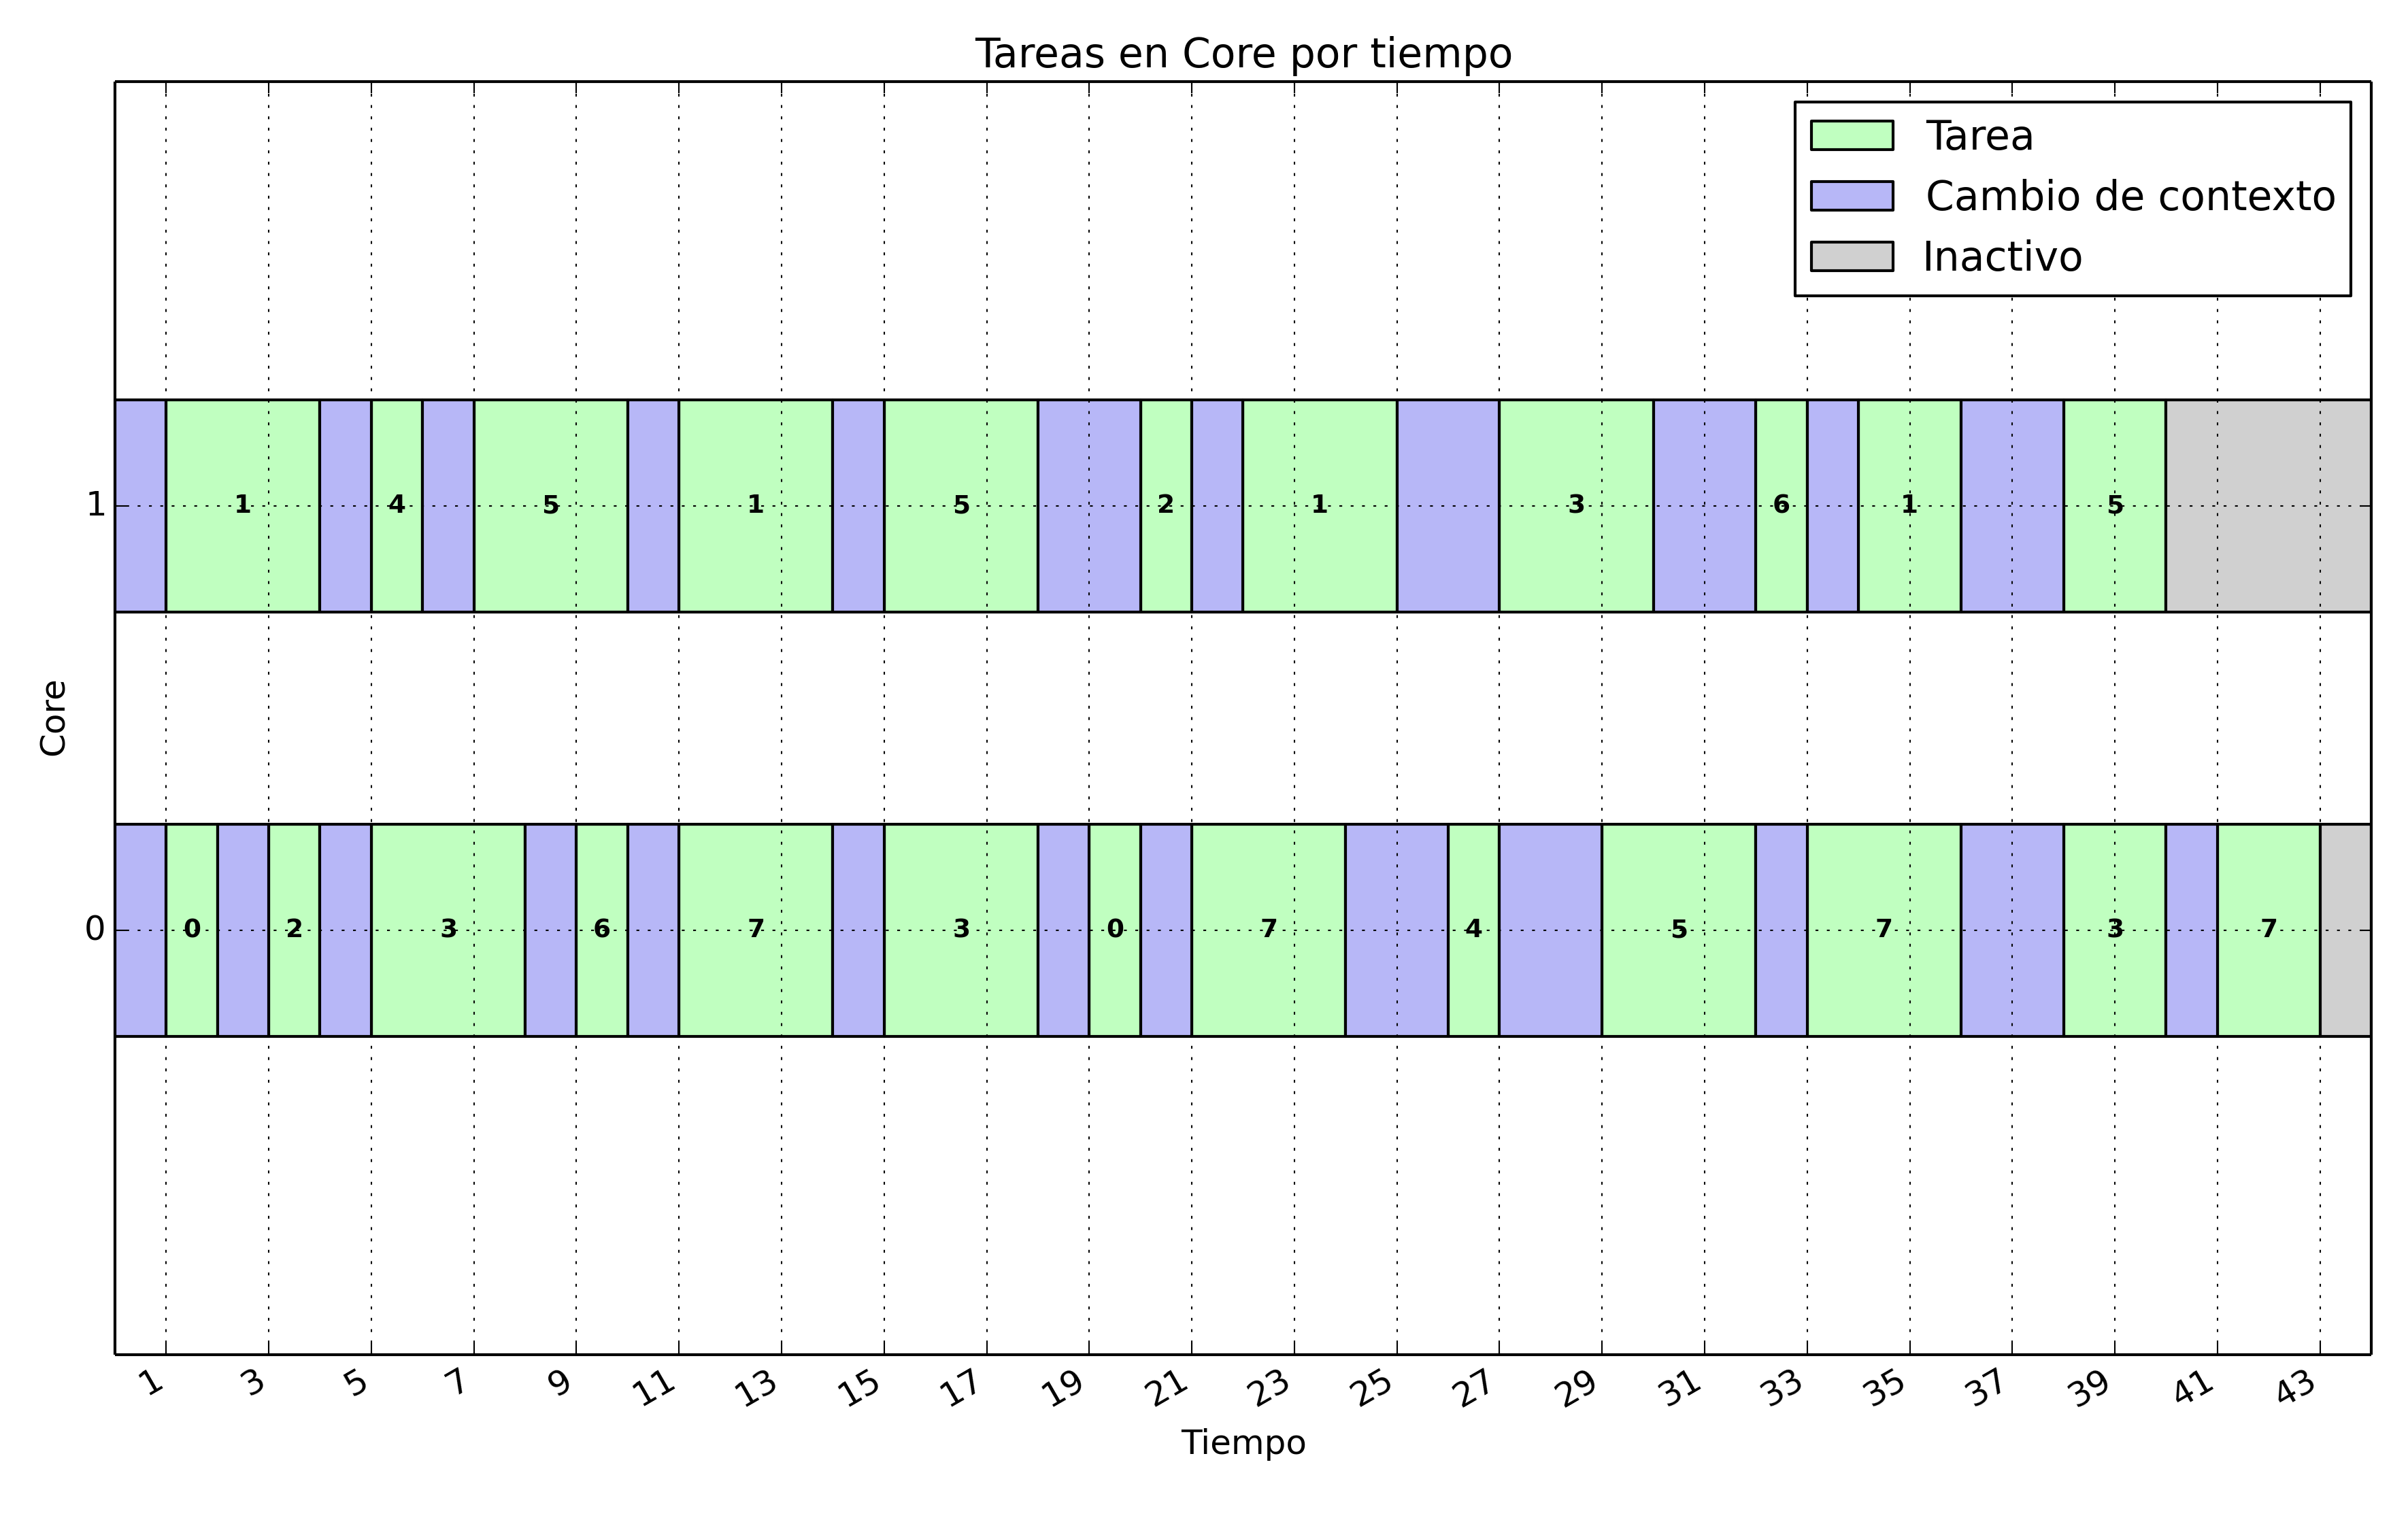
\includegraphics[scale=.4, width=1\textwidth]{graficos/ej8-a1-2c-cores}
		\caption{SchedRR (con migración) - Uso de cores}
		\end{figure}
		
		\begin{figure}[H]
		\centering
		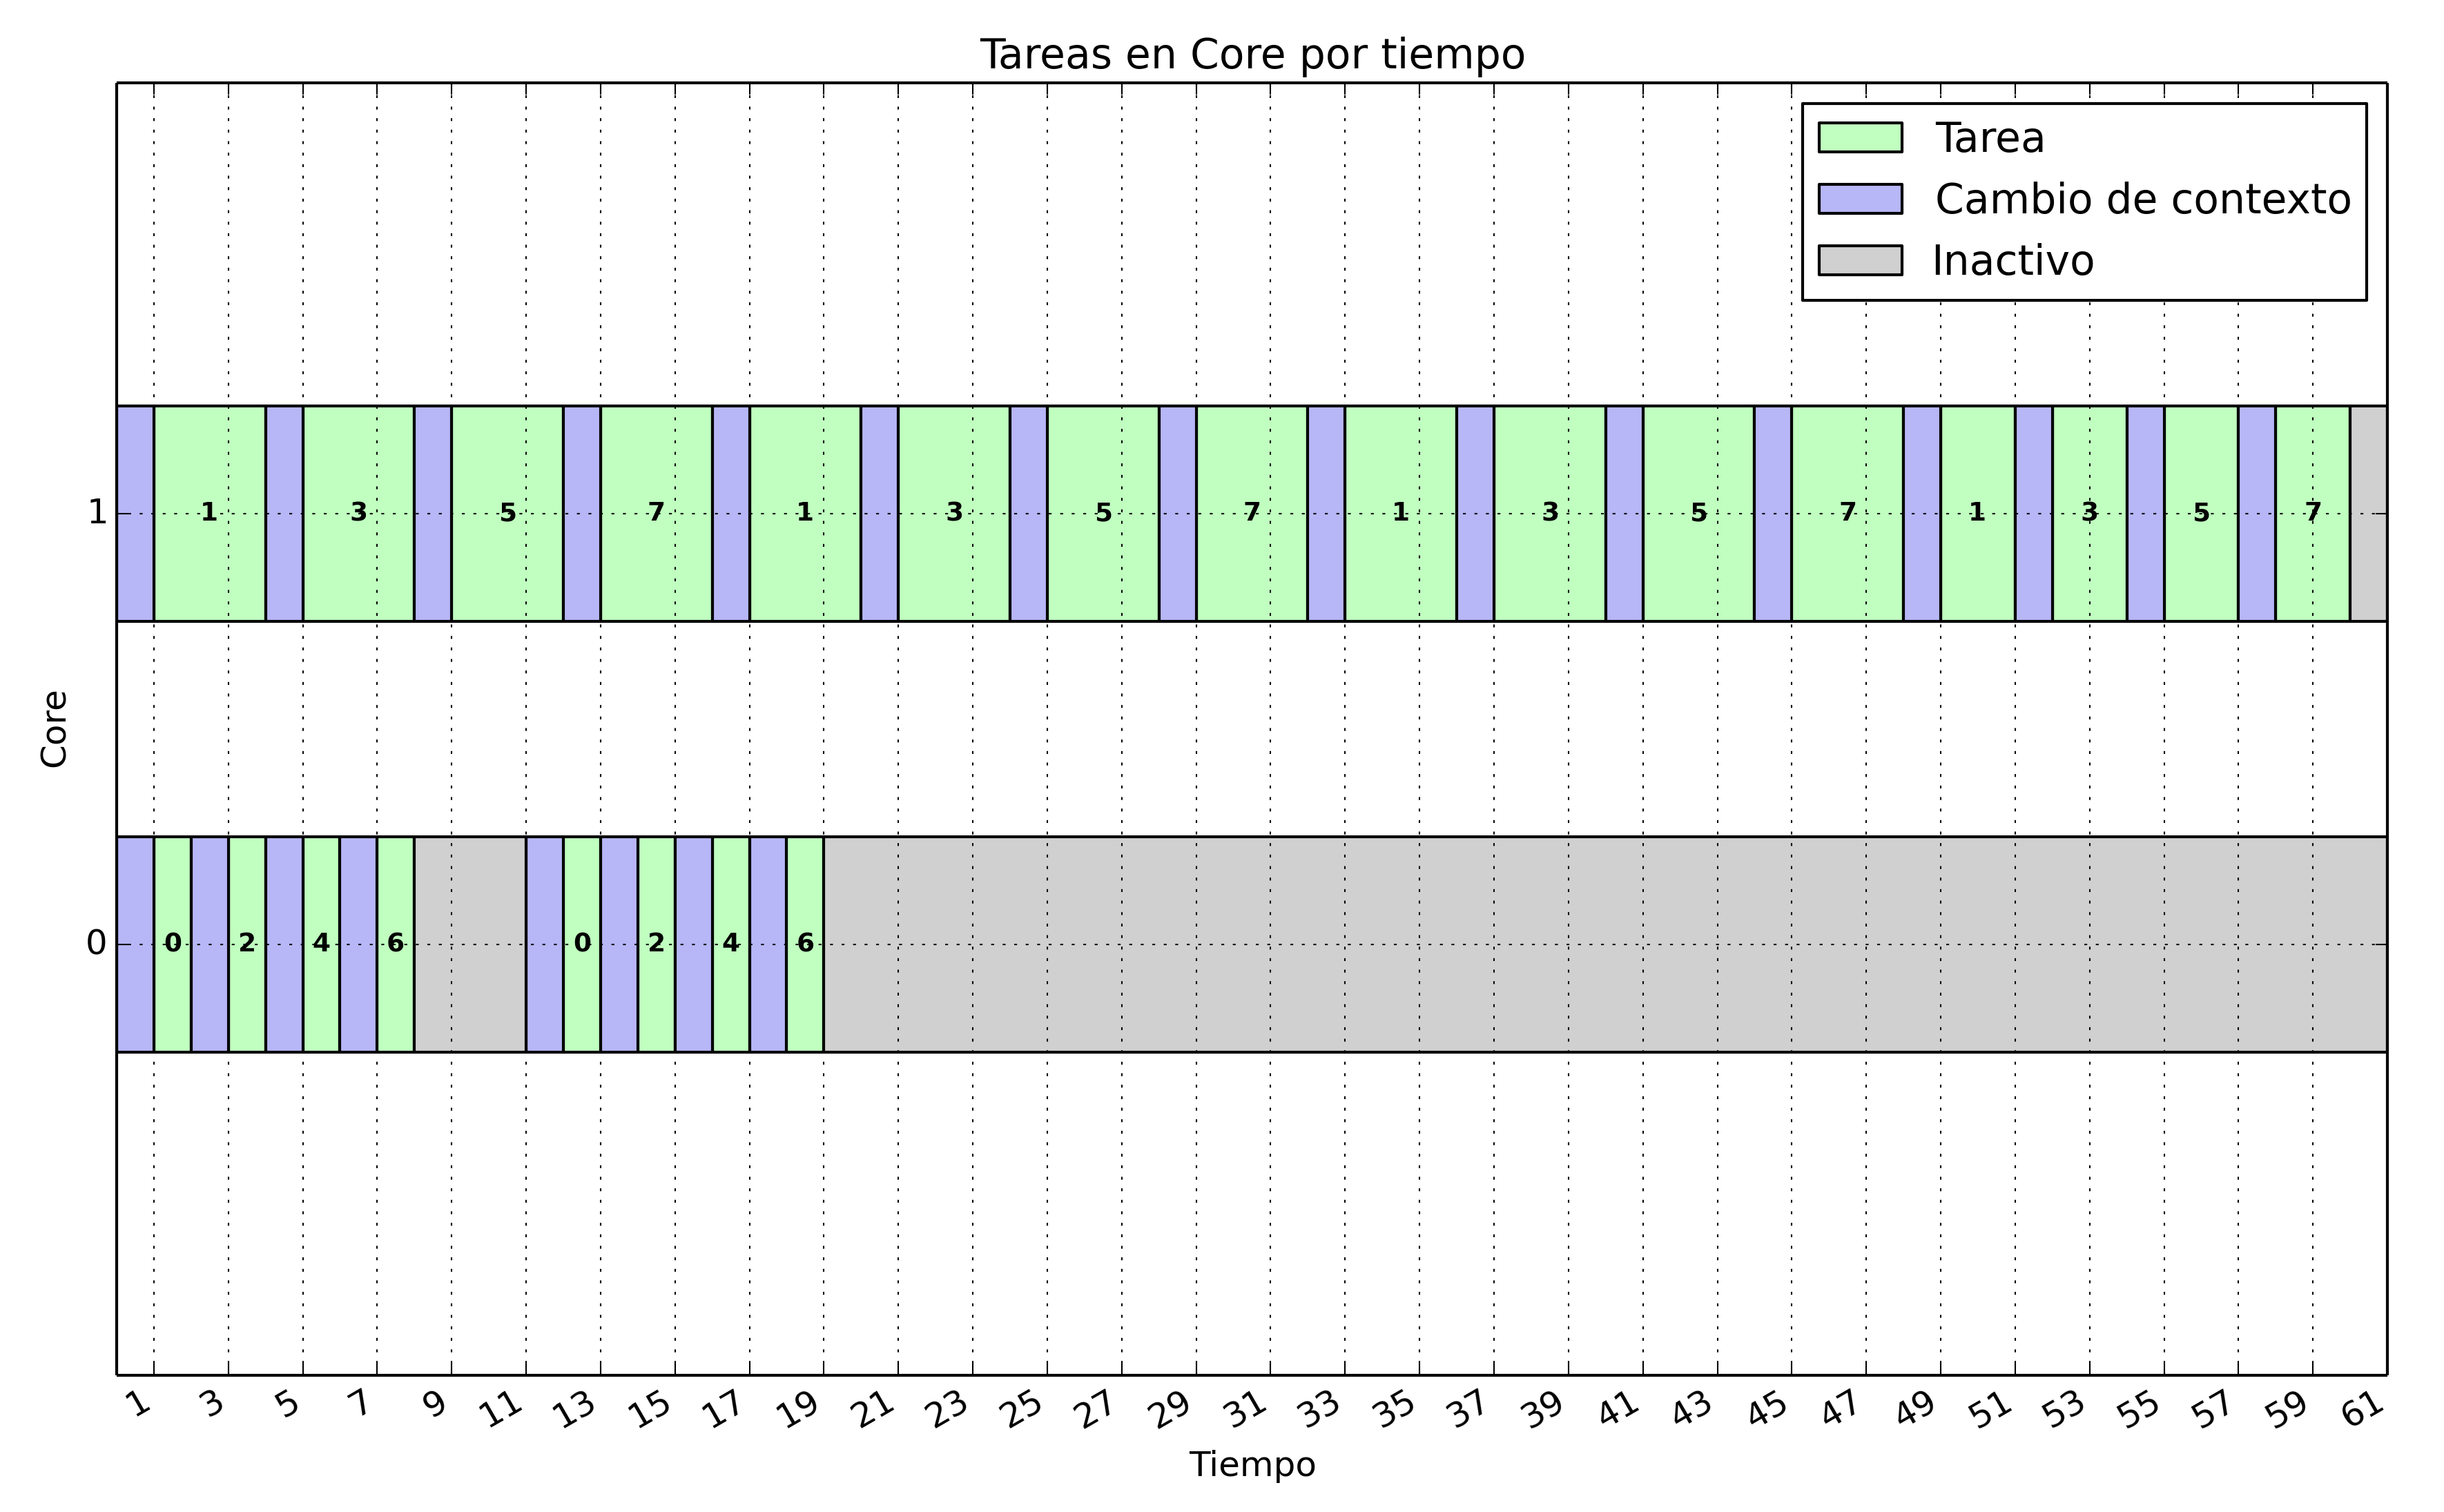
\includegraphics[scale=.4, width=1\textwidth]{graficos/ej8-a2-2c-cores}
		\caption{SchedRR2 (sin migración) - Uso de cores}
		\end{figure}	

		Como esperabamos es notoria la diferencia entre el uso que estos algoritmos hacen de sus cores. Para la implementación sin migración podemos ver que gran parte del tiempo uno de los cores está inactivo mientras espera a que las tareas se desbloqueen, tal y como habíamos previsto.
		
		\subsubsection{Experimento 2}
		

\section{Ejercicio 9}

Para diseñar este lote de tareas, tuvimos en cuenta la sección 9 del paper en la que se analiza el \emph{Utilization Factor} que se define como:

\begin{center}
$\displaystyle U = \sum_{i=0}^{m} \left(\frac{C_i}{T_i}\right) $
\end{center}
Siendo \emph{m} la cantidad de familias de tareas, \emph{C} el tiempo de procesamiento y \emph{T} el período de cada familia.

El paper propone el siguiente ejemplo:
\begin{center}
$C_1 = C_2 = 1$, $C_3 = 2$, $T_1 = 3$, $T_2 = 4$ y $T_3 = 5$
\end{center}
en el cual $U = 98\% $ para el scheduler de prioridades dinámicas y asegura que para que ese set de tareas sea factible en el scheduler de prioridades fijas, $C_3 \leq 1$. Con lo cual si diseñamos un lote de tareas que cumpla con estas características, nos aseguramos que va a ser factible para prioridades dinámicas y no para fijas. Por lo tanto proponemos el siguiente lote de tareas:
\begin{center}
$C_1 = 3$, $ C_2 = 2$, $C_3 = 2$, $T_1 = 9$, $T_2 = 8$ y $T_3 = 5$
\end{center}
para el cual el \emph{Utilization Factor} se mantiene en $98\%$ y no se produce overflow, por lo tanto es factible. El siguiente gráfico muestra la ejecución de las tareas utilizando prioridades dinámicas.
\begin{figure}[H]
\centering
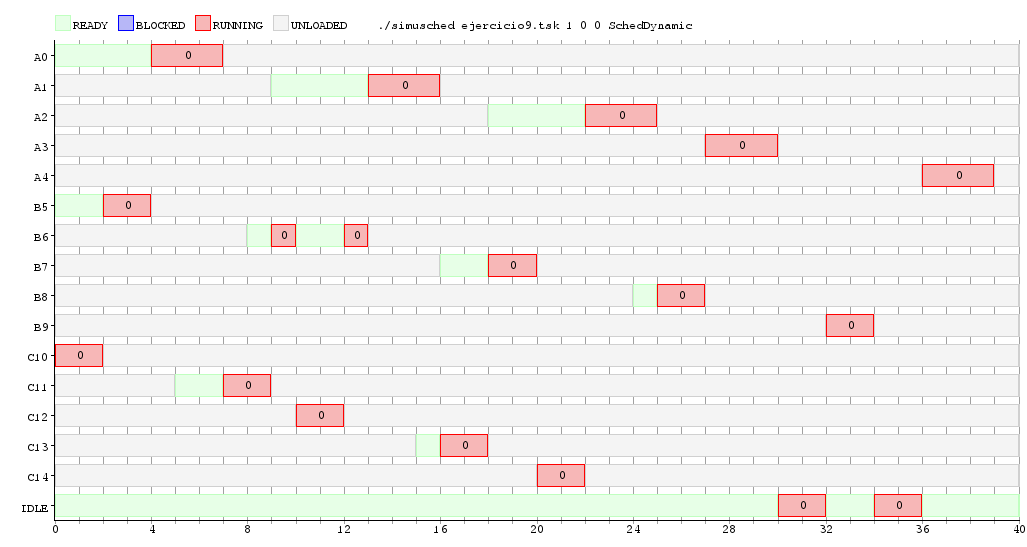
\includegraphics[scale=.6, width=1\textwidth]{graficos/ej9-dyn}
\caption{Lote de tareas con prioridades dinámicas}
\end{figure}
Como se puede observar, las tareas logran completarse antes de que llegue la próxima tarea de la misma familia. En cambio, al intentar utilizar este lote de tareas con el scheduler de prioridades fijas, sin adaptar $C_3$, se puede observar, en el gráfico que sigue, que se produce overflow en el instante 9 para la tarea A0 con la A1 y en el instante 18 entre las tareas A1 y A2. Esto ocurre porque al tener prioridad fija en el período, las tareas de la familia A siempre pierden contra las de las familias B y C, que tienen período mas corto y no se tiene en cuenta hace cuanto llegó una tarea, lo que provoca que haya tareas muy cerca del deadline a las cuales no se les asigna tiempo de procesador con suficiente anticipación para que pueda terminar de ejecutar antes de que llegue la tarea siguiente. Por lo tanto este bloque de tareas no es factible para este tipo de scheduler.  
\begin{figure}[H]
\centering
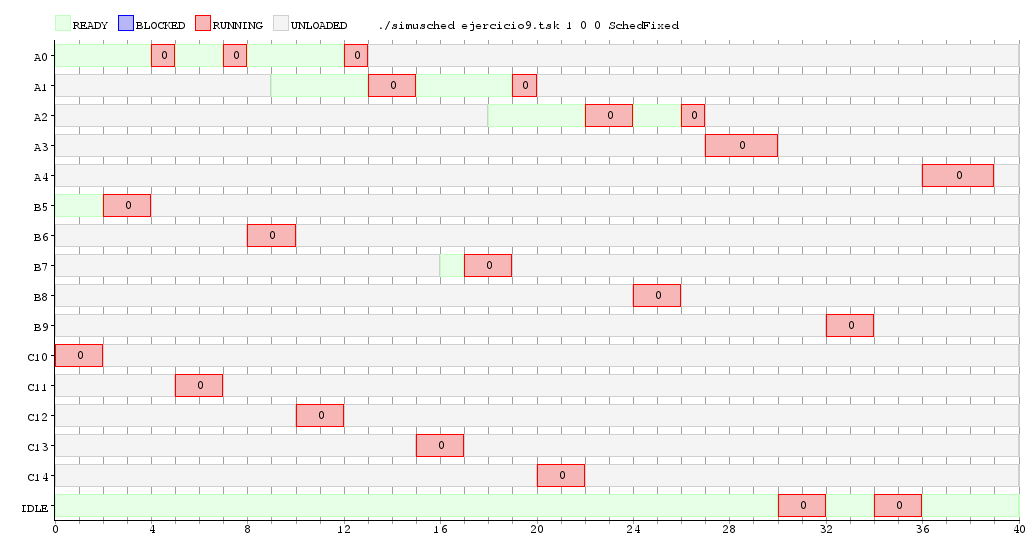
\includegraphics[scale=.6, width=1\textwidth]{graficos/ej9-fix}
\caption{Lote de tareas con prioridades fijas}
\end{figure}


\end{document}

